\documentclass[11pt]{article}

\usepackage[margin=1in]{geometry}
\usepackage{graphicx}
\usepackage{booktabs}
\usepackage{hyperref}
\usepackage{enumitem}
\setlist{itemsep=0.25em,topsep=0.4em}
\hypersetup{colorlinks=true,linkcolor=black,urlcolor=blue}

\title{DAT 5668 \\ Module 1 Notes \\ The Agent Loop}
\author{Salih Tutun, PhD \\ Olin Business School \\ Washington University in St.\ Louis}
\date{Fall 2026}

\begin{document}
\maketitle

\begin{abstract}
\noindent
These notes are the reading for Module 1. Session~1 teaches the idea in the room. Session~2 is where you build the tool-using agent. Open \texttt{Session-01.ipynb} and \texttt{Session-02.ipynb} beside this document. The figures are the same ones in the notebooks. There is no recording to watch first.
\end{abstract}

\section{What an agent is}

An agent acts toward a goal in an environment. The definition is the loop, not the brand of the model.

\begin{center}
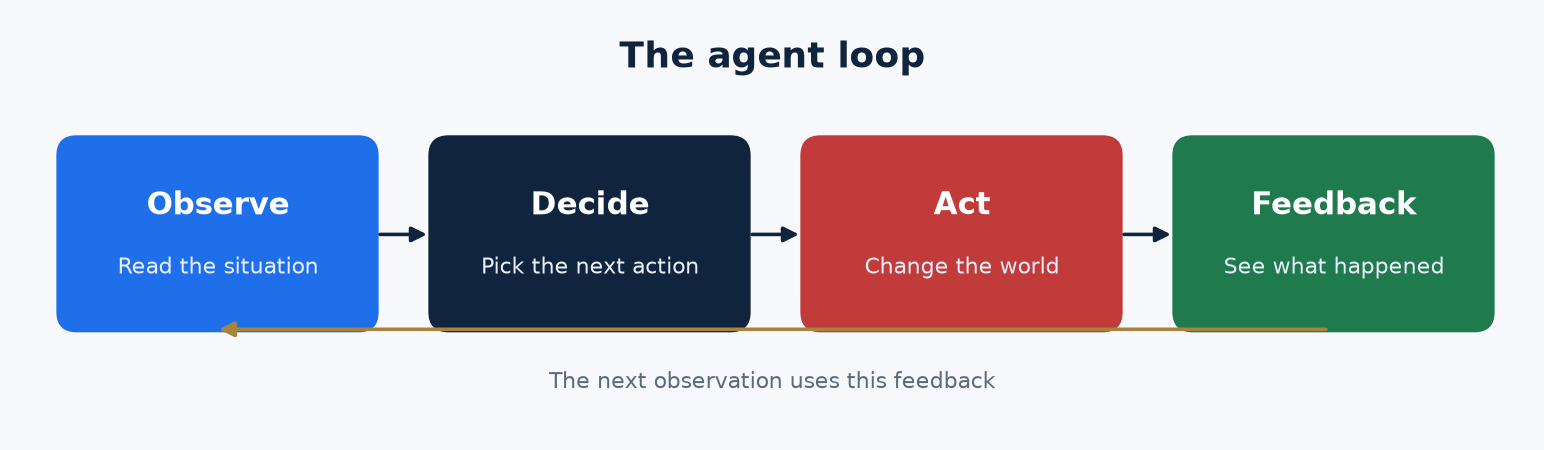
\includegraphics[width=0.92\textwidth]{../../assets/agent-loop.png}
\end{center}

\begin{center}
\begin{tabular}{@{}llp{7.2cm}@{}}
\toprule
Step & Meaning & Refund desk \\
\midrule
Observe & Read the situation & Ticket text, order age, order total \\
Decide & Pick the next action & Look up the policy, then approve, refuse, or escalate \\
Act & Change something outside the model & Post the refund or open a case \\
Feedback & See whether the action helped & The amount came from the order record, and a person can audit the tools \\
\bottomrule
\end{tabular}
\end{center}

A chatbot that only writes a polite paragraph is not yet an agent. It never took an action the desk can audit, and it has no feedback tied to the order. The refund amount has to come from the system of record. The model does not invent a dollar figure.

\section{Two families, one loop}

\begin{center}
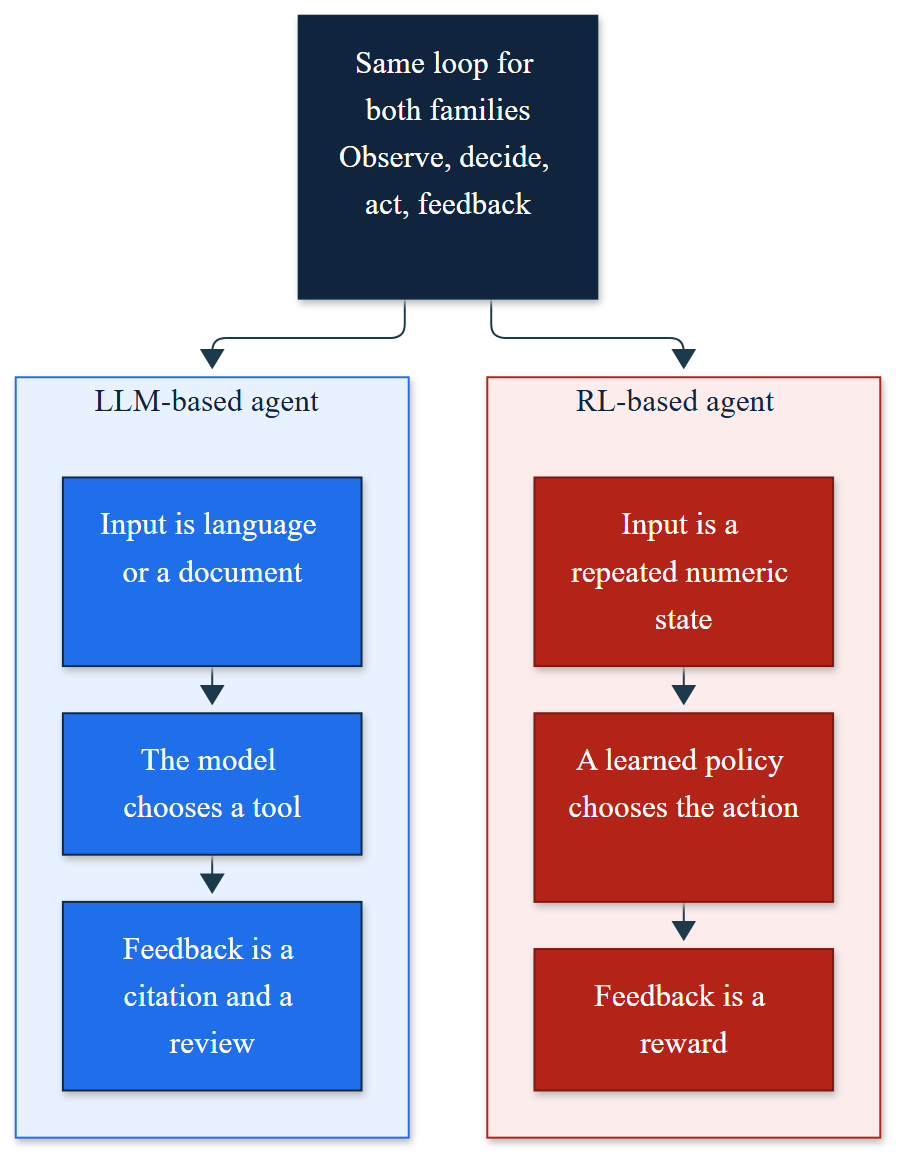
\includegraphics[width=0.78\textwidth]{../../assets/two-families.png}
\end{center}

An LLM-based agent and an RL-based agent answer the same managerial question with different machinery.

\begin{itemize}
\item An \textbf{LLM-based agent} reads language or a document, chooses a tool, and is checked by a citation and a review.
\item An \textbf{RL-based agent} reads a repeated numeric state, chooses an action from a learned value, and is checked by a reward.
\end{itemize}

Using the wrong family is a design error. A chat reply is a poor inventory controller: the state is stock, the action is an order quantity, and the feedback is a number that repeats. A deep Q-network is a poor contract reviewer: the input is unstructured language, and the action is a tool call plus a reason a person can check.

Session~1 runs both families on the same tickets so you can see where they agree and where they do not. The RL family is trained later, starting in Session~4. Session~1 only shows a small learned table.

\section{The same three tickets}

The case is instructional. It is not data from a firm. The policy the business will stand behind is short:

\begin{itemize}
\item A damaged item may be refunded within 30 days.
\item An order older than 30 days is refused unless a manager escalates.
\item ``Changed my mind'' is not a damage claim. The policy tool refuses it.
\item The refund amount is the order total.
\end{itemize}

\begin{center}
\begin{tabular}{@{}clcc@{}}
\toprule
Ticket & Text & Age (days) & Total \\
\midrule
A & Item arrived cracked & 12 & \$80 \\
B & Changed my mind & 10 & \$40 \\
C & Screen is cracked & 45 & \$200 \\
\bottomrule
\end{tabular}
\end{center}

\subsection{The language-model side}

The decide step may name only three tools: \texttt{lookup\_policy}, \texttt{lookup\_amount}, and \texttt{finish}. It may not invent a fourth tool, and it may not invent the dollar amount. \texttt{lookup\_amount} reads the order total. \texttt{finish} returns refund, refuse, or escalate.

In class the decide step is a local stand-in, so the notebook runs with no API key. If a Gemini key is set, that same step can ask Gemini which tool to call next. The tools still run in the notebook. A missing key, a refused call, or a tool name outside the schema falls back to the stand-in. Do not paste a firm secret into the ticket text.

On these three tickets the stand-in refunds A, refuses B, and refuses C. Ticket~C is damaged, but it is outside the 30-day window.

\subsection{The reinforcement-learning side}

The RL agent does not read the sentence. A small mapping turns the ticket into a state: fresh damage, stale damage, or other. It then picks the action with the largest learned value. Actions are refund, refuse, and escalate.

Ticket~B is the point of the session. The language-model agent refuses it, because the policy tool says a change of mind is not eligible. The RL agent has no damage rule for that sentence, so the state is ``other,'' and the learned table escalates. That disagreement is a design fact. It is not a bug in the code.

\section{What to say to a manager}

Ask these five questions before anyone builds the agent. They are the same questions for both families.

\begin{enumerate}
\item \textbf{Goal.} What decision, if automated, would change a KPI this quarter?
\item \textbf{Data.} Is the input a document or ticket, or a repeated numeric state?
\item \textbf{Actions.} What may the system do, and what is forbidden?
\item \textbf{Feedback.} Is the signal a citation and a human rating, or a numeric reward every step?
\item \textbf{Human checkpoint.} Which action is too costly to take without a person?
\end{enumerate}

Inside the policy window, a damaged item can be auto-approved. ``Other'' should be seen by a person. Neither family should override the 30-day window.

\section{Session 2: from a chatbot to an agent}

\begin{center}
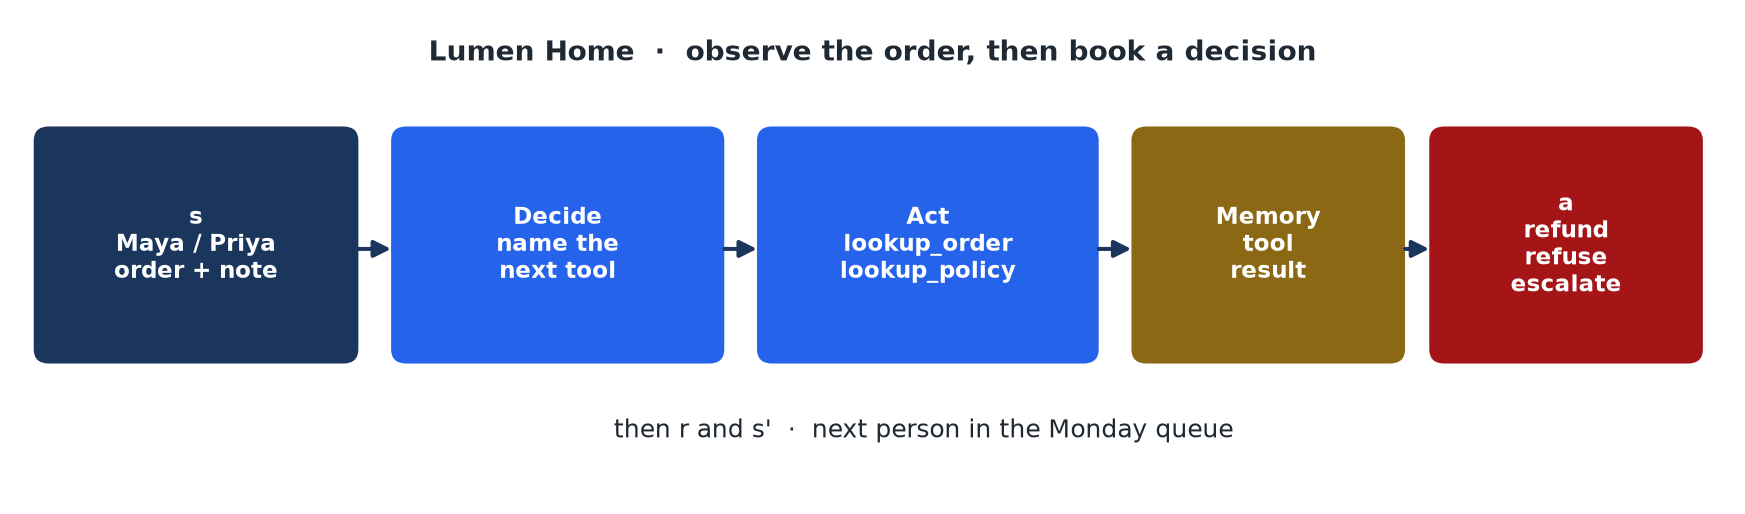
\includegraphics[width=\textwidth]{../../assets/llm-tool-loop.png}
\end{center}

Session~2 is the practice session. You build the language-model side. The business rule is the same: refund a damaged item only when the order is 30 days old or newer, and take the amount from the order record.

A chatbot cell in the notebook refunds an invented \$999. That cell is the failure mode. Your \texttt{decide} function has to beat it.

\begin{enumerate}
\item Observe the order with \texttt{lookup\_order}. An unknown id escalates.
\item Observe the rule with \texttt{lookup\_policy} on the order note.
\item Refund only when the reason is eligible and the age is inside the window. Otherwise refuse.
\item If the order is missing, escalate and call \texttt{open\_case}.
\item The refund amount equals the order total. Do not hard-code 999.
\end{enumerate}

The function returns \texttt{action}, \texttt{amount}, \texttt{reason}, and \texttt{case\_id}. Groups in the room may be 1--3 students. The homework after class is individual.

\subsection{The homework rule}

Homework~1 adds one rule to the Session~2 agent. If the order total is above \$150, do not auto-refund. Escalate and open a case. The rest of the policy stays as it was.

\section{What you should be able to say}

\begin{itemize}
\item The loop is observe, decide, act, feedback.
\item A fluent email with no tool call is not an agent.
\item Name one job for an LLM-based agent and one job for an RL-based agent.
\item Say why a chatbot is a poor inventory controller.
\item Name the fifth managerial question: the human checkpoint.
\end{itemize}

Quiz~1 covers this session. It is the multiple-choice quiz on Canvas, due one hour before Session~2. A late quiz is not accepted except with an excused absence.

\end{document}
